\documentclass[12pt]{article}
\usepackage[margin=1in, bottom = 1.5in]{geometry} 
\usepackage{amsmath,amsthm,amssymb,amsfonts, enumitem, float, fancyhdr, color, comment, graphicx, environ,setspace, subcaption, lastpage, tabularx, booktabs, caption}
\captionsetup[subfigure]{width=0.85\linewidth}
\usepackage{tikz}
\usetikzlibrary{calc}
\pagestyle{fancy}
\fancyhf{}
\lhead{Galois Theory for Rats}  
\rhead{Compass \& Straightedge Construction}
\fancyfoot[R]{Page \thepage\ of \pageref{LastPage}}
\newlength{\myfootheight}
\setlength{\myfootheight}{35pt} 
\renewcommand{\footrulewidth}{0.4pt}
\setlength{\headheight}{35pt}
\pagenumbering{arabic}


% Define the theorem, lemma, proposition and corollary environmentsc

\newtheorem{corollary}{Corollary}[section]
\theoremstyle{definition}
\newtheorem{definition}{Definition}[section]
\theoremstyle{definition}
\newtheorem{example}{Example}[section]
\theoremstyle{definition}
\newtheorem{theorem}{Theorem}[section]
\theoremstyle{definition}
\newtheorem{lemma}{Lemma}[section]
\theoremstyle{definition}
\newtheorem{proposition}{Proposition}[section]
\theoremstyle{definition}


\AtBeginDocument{%
  \mathchardef\stdcomma=\mathcode`,
  \mathcode`,="8000
}
\begingroup\lccode`~=`, \lowercase{\endgroup\def~}{\stdcomma\,}

\title{Galois Theory for Rats - Compass \& Straightedge Construction}
\author{Skyler Hu}

\begin{document}
\linespread{1.05}
\maketitle
\newpage
\tableofcontents
\newpage

\begin{section}{Motivation \& Construction Axioms}
    Initially,field theory and Galois Theory was all about solving ancient problems deemed unsolvable (in case of the quintic) so it is
    no surprise that it could be used to explain another collection of classic problems, that of compass and straightedge constructions.
    The notion of compass and straightedge constructions is usually introduced early on in math courses -- we learned the basics of construction
    including constructing paralle lines, constructing the angle bisector of an angle and the perpendicular bisector of a line segment. There are nuanced differences between 
    `construction' problems we encountered in high school and `construction' problems as accepted in field theory, so it serves us to first define 
    what a compass and straightedge are and what can they do.

    \begin{definition}{(Compass \& Straightedge)}
        A straightedge, unlike a ruler, has no measure of length. A compass is defined conventionally.
    \end{definition}

    \begin{definition}{(Operations in Compass \& Straightedge Construction)}
        In compass and straightedge construction, one can only do the three following operations:
        \begin{enumerate}
            \item Draw a line through two given points;
            \item Draw a circle centered at a given point and passing through another given point (i.e. given center and radius);
            \item Obtain the point of intersection of a line and a circle or of two circles.
        \end{enumerate}
        \textbf{Note.} A common mistake here is to assume that a compass \textit{can preserve distance} -- that is, one can copy a line segment of a 
        given distance by aligning two ends of the compass to each end of the line segment. In the original (and classic) case of the construction problem
        posed by Euclid, a \textit{collapsing} compass is used, one that would collapse when you pick it up. This is for two reasons: \textbf{(a)} Euclid
        made the fewest possible assumptions about the functions of a compass and straightedge, and \textbf{(b)} it is doubtful that the ancient Greeks had 
        in their possession modern rigid compasses. \\
        Despite this, it can be proved that the two compasses are equal in construction: what one could do, the other also could. A detailed explanantion is
        included in the Proofs and Further Reading section.
    \end{definition}

    The proofs of this section aren't too difficult, so it is advised to work through them with a compass and straightedge if possible. The construction problems 
    date back thousands of years and the resolution is extremely satisfying -- have fun!
\end{section}

\newpage

\begin{section}{The Four Operations, plus one}
    When delving into compass and straightedge construction, we are most concerned about which lengths can be constructed from the unit length (1). The defintion 
    of constructibility helps us formalize this.

    \begin{definition}{(Constructibility)}
        A positive real number \(m\) is \textit{constructible} if a line segment of length \(m\) can be constructed with compass and straightedge from a line segment 
        of length 1, otherwise it is not constructible.
    \end{definition}

    We might expect the compass and straightedge to be able to perform the four operations, addition, subtraction, multiplication and division. This is true, and 
    we can prove it!

    \begin{theorem}{(The Four Operations.)}
        Given constructible lengths \(a\) and \(b\), the lengths \(a+b, a-b, ab\) and \(a/b\) are all constructible.
        \begin{proof}
            We'll need the following elementary result:
            \begin{lemma}
                If \(a\) is constructible, then we can obtain on the plane the point \((a,0)\) located on the \(x\)-axis. Generally, if \(a\) is constructible, then we 
                can obtain a line segment of length \(a\) anywhere on the plane. \\
                \noindent\textbf{Note.} We might consider this statement trivial, but in Euclid's original defintion that uses a collapsing compass (non-distance preserving)
                this statement needs a rigorous proof. Details in the Proofs \& Further Reading section. In the meantime, we can assume this is true.
            \end{lemma}

            The following proofs are geometric, so assume that \(a,b\) are positive and \(a>b\) to avoid negative lengths.\\

            \noindent\textbf{1. Addition and Subtraction.} This is easy. Construct a circle centered at \((a,0)\) with radius \(b\).
            \begin{figure}[h!]
                \centering
                \begin{tikzpicture}[>=stealth, thick, scale=1.2]                   
                    \newcommand{\dimline}[4]{
                        \draw ($(#1)+(0,#4)$) -- ($(#1)+(0,#4-0.2)$);
                        \draw ($(#2)+(0,#4)$) -- ($(#2)+(0,#4-0.2)$);
                        \draw ($(#1)+(0,#4-0.1)$) -- ($(#2)+(0,#4-0.1)$) 
                            node[midway, fill=white] {#3};
                    }

                    \def\a{4}
                    \def\b{1.5}
                    
                    \coordinate (O) at (0,0);
                    \coordinate (A) at (\a,0);
                    \coordinate (L) at (\a-\b,0);
                    \coordinate (R) at (\a+\b,0);
                    
                    \draw (O) -- (A);
                    \draw (A) circle (\b);
                    \draw (A) -- ++(45:\b) node[midway, above, sloped] {$b$};
                    \draw (A) -- (R);

                    \fill (O) circle (0.05) node[below] {$O$};
                    \fill (A) circle (0.05) node[below] {$A$};
                    
                   
                    \dimline{O}{A}{$a$}{+0.1}
                    \dimline{L}{A}{$a-b$}{-0.5}   
                    \dimline{O}{R}{$a+b$}{-1.0}   
                \end{tikzpicture}
                \caption{Addition \& Subtraction}
                \end{figure}


                \noindent\textbf{2. Multiplication.} Consider constructing similar triangles. 
                \begin{figure}[H]
                \centering
                \begin{tikzpicture}[thick, scale=1.5]

                    \newcommand{\dimline}[4]{
                        \draw ($(#1)+(0,#4)$) -- ($(#1)+(0,#4-0.15)$);
                        \draw ($(#2)+(0,#4)$) -- ($(#2)+(0,#4-0.15)$);
                        \draw ($(#1)+(0,#4-0.08)$) -- ($(#2)+(0,#4-0.08)$)
                            node[midway, fill=white, font=\small] {#3};
                    }

                    \coordinate (O) at (0,0);

                   
                    \coordinate (A) at (1,0);     
                    \coordinate (B) at (0,1.2);   

                    \def\a{2}
                    \coordinate (C) at (\a,0);    
                    \coordinate (D) at (0,\a*1.2); 

                    \draw (O) -- (A) -- (B) -- cycle;  % △OAB
                    \draw (O) -- (C) -- (D) -- cycle;  % △OCD

                    \fill (O) circle (0.04) node[below left] {$O$};
                    \fill (A) circle (0.04) node[below] {$A$};
                    \fill (B) circle (0.04) node[above left] {$B$};
                    \fill (C) circle (0.04) node[below] {$A_1$};
                    \fill (D) circle (0.04) node[left] {$B_1$};
                    \dimline{O}{A}{$1$}{-0.4}

                    \dimline{O}{C}{$a$}{-0.8}


                    \draw ($(O)+(-0.4,0)$) -- ($(O)+(-0.25,0)$);
                    \draw ($(B)+(-0.4,0)$) -- ($(B)+(-0.25,0)$);
                    \draw ($(O)+(-0.325,0)$) -- ($(B)+(-0.325,0)$)
                        node[midway, fill=white, font=\small] {$b$};


                    \draw ($(O)+(-0.9,0)$) -- ($(O)+(-0.75,0)$);
                    \draw ($(D)+(-0.9,0)$) -- ($(D)+(-0.75,0)$);
                    \draw ($(O)+(-0.825,0)$) -- ($(D)+(-0.825,0)$)
                        node[midway, fill=white, font=\small] {$ab$};

                \end{tikzpicture}
                \caption{$\triangle OAB \sim \triangle OA_1 B_1$}
            \end{figure}
            Construct from the origin \(O\) line segments \(OA=1\) and \(OA_1 =a\). Construct a circle centered 
            at \(O\) with radius \(b\), pick an arbitrary point \(B\) on the circle, then \(OB=b\). Construct line segment 
            \(A_1 B_1// AB\) such that \(B_1\) is on line \(OB\). Then \(OB_1 = ab\).\\
            \break

            \noindent\textbf{3. Division.} Similar to the proof for multiplication, we construct two similar triangles with 
            slightly different side lengths:

            \begin{figure}[H]
                \centering
                \begin{tikzpicture}[thick, scale=1.5]

                    \newcommand{\dimline}[4]{
                        \draw ($(#1)+(0,#4)$) -- ($(#1)+(0,#4-0.15)$);
                        \draw ($(#2)+(0,#4)$) -- ($(#2)+(0,#4-0.15)$);
                        \draw ($(#1)+(0,#4-0.08)$) -- ($(#2)+(0,#4-0.08)$)
                            node[midway, fill=white, font=\small] {#3};
                    }

                    \coordinate (O) at (0,0);

                   
                    \coordinate (A) at (1,0);     
                    \coordinate (B) at (0,1.2);   

                    \def\a{2}
                    \coordinate (C) at (\a,0);    
                    \coordinate (D) at (0,\a*1.2); 

                    \draw (O) -- (A) -- (B) -- cycle;  % △OAB
                    \draw (O) -- (C) -- (D) -- cycle;  % △OCD

                    \fill (O) circle (0.04) node[below left] {$O$};
                    \fill (A) circle (0.04) node[below] {$B_1$};
                    \fill (B) circle (0.04) node[above left] {$A_1$};
                    \fill (C) circle (0.04) node[below] {$B$};
                    \fill (D) circle (0.04) node[left] {$A$};
                    \dimline{O}{A}{$1$}{-0.4}

                    \dimline{O}{C}{$b$}{-0.8}


                    \draw ($(O)+(-0.4,0)$) -- ($(O)+(-0.25,0)$);
                    \draw ($(B)+(-0.4,0)$) -- ($(B)+(-0.25,0)$);
                    \draw ($(O)+(-0.325,0)$) -- ($(B)+(-0.325,0)$)
                        node[midway, fill=white, font=\small] {$a/b$};


                    \draw ($(O)+(-0.9,0)$) -- ($(O)+(-0.75,0)$);
                    \draw ($(D)+(-0.9,0)$) -- ($(D)+(-0.75,0)$);
                    \draw ($(O)+(-0.825,0)$) -- ($(D)+(-0.825,0)$)
                        node[midway, fill=white, font=\small] {$a$};

                \end{tikzpicture}
                \caption{$\triangle OAB \sim \triangle OA_1 B_1$}
            \end{figure}
            Construct \(OB_1 = 1, OA=a, OB=b\). Construct line segment \(A_1 B_1 // AB\) with \(A_1\) on line \(OA\). Then 
            \(A_1 B_1 = a/b\).
        \end{proof}
    \end{theorem}

    Therefore addition, subtraction, multiplication and division are all valid operations in compass and straightedge construction. We 
    know that these aren't the only valid operations, though; take for example the fact that \(\sqrt{2}\) is constructible.\\
    \begin{figure}[H]
        \centering
        \begin{tikzpicture}[thick, scale=2]

            \coordinate (A) at (0,0);
            \coordinate (B) at (1,0);
            \coordinate (C) at (1,1);
            \coordinate (D) at (0,1);

            \draw (A) -- (B) -- (C) -- (D) -- cycle;
            \draw (A) -- (C);

            \node at (0.5, -0.2) {$1$};
            \node at (0.4, 0.7) {$\sqrt{2}$};

        \end{tikzpicture}
        \caption*{\(\sqrt{2}\) is the diagonal of a square of side length 1.}
    \end{figure}

    We can conclude that some roots are constructible. The constructible roots are none other than the square root, and we have the following:
    \begin{theorem}{(Square root)}
        If \(a\) is a positive constructible real number, then \(\sqrt{a}\) is also constructible.
        \begin{proof}
            This one is slightly trickier and uses the elementary result that the angle subtended by the diameter is \(90^{\circ}\) (and also 
            similar triangles).
            \begin{figure}[h!]
                \centering
                \begin{tikzpicture}[thick, scale=1.8]

                    \newcommand{\dimline}[4]{
                        \draw ($(#1)+(0,#4)$) -- ($(#1)+(0,#4-0.15)$);
                        \draw ($(#2)+(0,#4)$) -- ($(#2)+(0,#4-0.15)$);
                        \draw ($(#1)+(0,#4-0.08)$) -- ($(#2)+(0,#4-0.08)$)
                            node[midway, fill=white, font=\small] {#3};
                    }

                    \def\a{2}          
                    \def\aplusone{3}   
                    
                    \coordinate (O) at (0,0);          
                    \coordinate (A) at (\a,0);         
                    \coordinate (B) at (\aplusone,0);  
                    \coordinate (C) at (\aplusone/2,0); 
                    
                    \draw (O) -- (B);
                    
                    \draw (O) arc[start angle=180, end angle=0, radius=\aplusone/2];
                    
                    \coordinate (P) at (\a,0);        
                    \coordinate (Q) at ({\a}, {sqrt(\a)}); 
                    
                    \draw[thick] (P) -- (Q);
                    \node at ({\a+0.25}, {sqrt(\a)/2})  {$\sqrt{a}$};
                    
                    \dimline{O}{A}{$a$}{-0.5}
                    \dimline{A}{B}{$1$}{-0.5}

                    \draw[dashed] (Q) -- (O);
                    \draw[dashed] (Q) -- (B);

                    \fill (A) circle (0.04) node[below] {$A$};
                    \fill (B) circle (0.04) node[below] {$B$};
                    \fill (O) circle (0.04) node[below] {$C$};
                    \fill (Q) circle (0.04) node[above] {$Q$};
                \end{tikzpicture}
                \caption{\(AQ \perp BC\)}
            \end{figure}
            Construct line segments \(AB=1, AC=a\) with \(A,B,C\) collinear. Construct a semicircle with diameter \(BC\), and 
            construct \(AQ \perp BC\) with \(Q\) on the semicircle. Then \(\angle BQC = 90^{\circ}\), so \(\triangle QAB \sim \triangle CQA\), 
            and \[\frac{AQ}{AB} = \frac{AC}{AQ},\] so \(AQ^2 = AB \cdot AC = a\). Therefore \(AQ = \sqrt{a}\).
        \end{proof}
    \end{theorem}

    By now we have a solid grasp of what operations are valid in compass and straightedge construction: the four operations, along with taking square 
    roots. In fact, we can show that these are the \textit{only} valid operations, with an argument of (surprisingly) analytic geometry. We can 
    formalize the `four operations \& square root' idea with field extensions:

    \begin{theorem}{(Degree of Extension from Compass \& Straightedge Construction.)}
        If the element \(\alpha \in F_k\) is obtained from field \(F\) through a series of compass and straightedge constructions, then \([F_k : F] = 2^k\)
        for some positive integer \(k\).
        \begin{proof}
            We analyze each of the 3 defined operations (see \textbf{Defintion 1.2}).\\
            \break
            \noindent\textbf{1. Finding the intersection of two lines.} A line in the plane with coordinates in \(F\) is of the form \(Ax + By + C =0\), 
            with coefficients all in \(F\). Solving for the intersection of two lines amounts to solving the simultaneous system of equations 
            \begin{align*}
                A_1 x + B_1 y + C_1 &= 0\\
                A_2 x + B_2 y + C_2 &= 0
            \end{align*}
            which has solutions also in \(F\).\\
            \break
            \noindent\textbf{2. Finding the intersection of a line and a circle.} A circle in the plane is of the form \((x-h)^2 + (y-k)^2 = r^2\) with 
            \(h,k,r \in F\). Solving for the intersection of a circle and a line amounts to solving the simultaneous system of equations
            \begin{align}
                Ax + By + C &= 0\\
                (x-h)^2 + (y-k)^2 &= r^2
            \end{align}
            Using the substitution \(x = -\frac{By+C}{A}\), we obtain from (2) a quadratic equation for \(y\) over \(F\). Therefore the solutions \(x,y\)
            are in an extension of degree at most 2 over \(F\).\\
            \break
            \noindent\textbf{3. Finding the intersection of two circles.} This is 
            \begin{align*}
                (x-h)^2 + (y-k)^2 &= r^2\\
                (x-h')^2 + (y-k')^2 &= r'^2
            \end{align*}
            Subtracting the two equations, we obtain a linear equation in terms of \(x\) and \(y\) (the quadratic terms cancel out). Then this case is the same as 
            finding the intersection of a line and a circle, and the solutions \(x,y\) are in an extension of degree at most 2 over \(F\).\\
            \break
            We can then conclude that compass and straightedge construction gives an extension of degree \(2^k\) over a base field \(F\).
        \end{proof}
        \noindent\textbf{Note.} This leads to the notion of the field of \textit{constructible numbers}, including all real numbers in an extension of degree 
        \(2^k\) over the integers (since the base field of compass and straightedge construction is generated by 1).
    \end{theorem}
\end{section}

\newpage

\begin{section}{The Classic Greek Construction Problems}
    Readers may have heard about (more or less) the three classic construction problems that have been troubling mathematicians since ancient times: 
    \begin{enumerate}
        \item (Duplicating the Cube.) Given a cube, can we construct a cube with twice its volume?
        \item (Trisecting the Angle.) Can we construct an angle that is 1/3 of a given angle?
        \item (Squaring the Circle.) Given a circle, can we construct a square with the same area?
    \end{enumerate}
    It turns out that none of these three questions have an affirmative answer, as is often the case with longstanding suspicious unsolved problems (see: quintic,
    a big chunk of G\"odel's work, parallel postulate) and we can disprove two of the three questions easily with what we've learned today! (You can take a guess at 
    which problem is a lot harder than the other two.)

    \begin{theorem}{(Classic Construction Problems.)}
        None of the classic Greek construction problems (duplicating the cube, trisecting the angle, squaring the circle) is achievable through compass and straightedge 
        construction.
        \begin{proof}
            \noindent\textbf{1. Duplicating the Cube.} This problem is equivalent to asking whether or not \(\sqrt[3]{2}\) is constructible, since a cube with volumne 2
            would have side length \(\sqrt[3]{2}\). Since \([\mathbb{Q}(\sqrt[3]{2}) : \mathbb{Q}] = 3\) which is not an integer power of 2, \(\sqrt[3]{2}\) is not constructible,
            and therefore it is impossible to obtain a cube with twice the volume of a given one with only compass and straightedge construction.\\
            \break
            \noindent\textbf{2. Trisecting the Angle.} If an angle \(\theta\) is constructible, then its cosine is constructible by finding the intersection of the angle and 
            the unit circle. Our problem then becomes: given \(\cos \theta\) is \(\cos \theta/3\) constructible?\\
            We can consider a special case (this is the most widely used argument for this problem): consider \(\theta = 60^{\circ}, \cos 60^{\circ} = 1/2\). We only need to show that \(\cos 20^{\circ}\)
            is not constructible. Using the triple-angle identity for cosine we obtain:
            \[\cos \theta = 4\cos^3 \theta/3 - 3\cos \theta/3.\]
            Substituting \(cos \theta/3 = x\) and \(cos 60^{\circ} = 1/2\), we have 
            \[4x^3 - 3x - 1/2 = 0 \Rightarrow (2x)^3 - 3(2x) - 1=0.\]
            Let \(y = 2x\). Then \(y^3 - 3y - 1=0\), and by the Rational Root Theorem the only possible rational root of this equation is \(-1\), which is apparently not a root of 
            \(y^3 - 3y - 1\). Therefore \(y^3 - 3y - 1\) is irreducible over \(\mathbb{Q}\), and its roots are in an extension of degree 3 over \(\mathbb{Q}\). Therefore \(y\) is not 
            constructible and neither is \(\cos 20^{\circ}\).\\
            \noindent\textbf{Note.} The proof shows that it is not generally possible to trisect the angle. However, we can certainly trisect \textit{some} angles, for example \(180^{\circ}\) and \(360^{\circ}\)
            (considering the regular hexagon which has an interior angle of \(120^{\circ}\) and an exterior angle of \(60^{\circ}\), both \(60^{\circ}\) and \(120^{\circ}\) are constructible). It turns out that 
            the only angles that are constructible are integer multiples of \(3^{\circ}\), for more details see the Proofs and Further Reading section.\\
            \break
            \noindent\textbf{3. Squaring the Circle.} A circle of radius 1 has area \(\pi\), so this question is equivalent to asking whether or not \(\pi\) is constructible. The argument for classifying \(\pi\)
            as transcendental is well beyond the scope of this handout, but here we shall assume that \([\mathbb{Q(\pi)} : \mathbb{Q}]\) is infinite, so \(\pi\) is not constructible and it is impossible to construct a 
            square with the area of a given circle. The proof of the transcendentality of \(pi\), unfortunately, is not included in the Proofs and Further Reading section because the author is also mystified. 
        \end{proof}
    \end{theorem}
\end{section}
\end{document}